\documentclass[
    xcolor={svgnames,dvipsnames},
    hyperref={colorlinks, citecolor=DeepPink4, linkcolor=DarkRed, urlcolor=DarkBlue}
]{beamer}  % for hardcopy add 'trans'

    %%%%%%%%%%%%%%%%%%%%% All document set up belongs here %%%%%%%%%%%%%%%%%%%%%
    \mode<presentation>
    {
      \usetheme{Singapore}
      % or ...
      \setbeamercovered{transparent}
      % or whatever (possibly just delete it)
    }
    \usepackage{fontspec}
    \usepackage{unicode-math}
    \setmonofont{DejaVu Sans Mono}[Scale=MatchLowercase] % provides unicode characters

    %%%%%%%%%%%%%%%%%%%%%% start my preamble %%%%%%%%%%%%%%%%%%%%%%
    \addtobeamertemplate{navigation symbols}{}{
        \usebeamerfont{footline}%
        \usebeamercolor[fg]{footline}%
        \hspace{1em}%
        \insertframenumber/\inserttotalframenumber
    }


    \usepackage{graphicx}
    \usepackage{amsmath, amssymb, amsthm}
    \usepackage{bbm}
    \usepackage{mathrsfs}
    \usepackage{xcolor}
    \usepackage{fancyvrb}


    % Quotes at start of chapters / sections
    \usepackage{epigraph}
    \renewcommand{\epigraphwidth}{6in}

    %% Fonts

    %\usepackage[T1]{fontenc}
    \usepackage{mathpazo}
    %\usepackage{fontspec}
    %\defaultfontfeatures{Ligatures=TeX}
    %\setsansfont[Scale=MatchLowercase]{DejaVu Sans}
    %\setmonofont[Scale=MatchLowercase]{DejaVu Sans Mono}
    %\setmathfont{Asana Math}
    %\setmainfont{Optima}
    %\setmathrm{Optima}
    %\setboldmathrm[BoldFont={Optima ExtraBlack}]{Optima Bold}

    % Some colors

    \definecolor{aquamarine}{RGB}{69,139,116}
    \definecolor{midnightblue}{RGB}{25,25,112}
    \definecolor{darkslategrey}{RGB}{47,79,79}
    \definecolor{darkorange4}{RGB}{139,90,0}
    \definecolor{dogerblue}{RGB}{24,116,205}
    \definecolor{blue2}{RGB}{0,0,238}
    \definecolor{bg}{rgb}{0.95,0.95,0.95}
    \definecolor{DarkOrange1}{RGB}{255,127,0}
    \definecolor{ForestGreen}{RGB}{34,139,34}
    \definecolor{DarkRed}{RGB}{139, 0, 0}
    \definecolor{DarkBlue}{RGB}{0, 0, 139}
    \definecolor{Blue}{RGB}{0, 0, 255}
    \definecolor{Brown}{RGB}{165,42,42}

    \setlength{\parskip}{1.5ex plus0.5ex minus0.5ex}

    %\renewcommand{\baselinestretch}{1.05}
    %\setlength{\parskip}{1.5ex plus0.5ex minus0.5ex}
    %\setlength{\parindent}{0pt}

    % Typesetting code
    \definecolor{bg}{rgb}{0.95,0.95,0.95}
    \usepackage{minted}
    \setminted{mathescape, frame=lines, framesep=3mm}
    \usemintedstyle{friendly}
    %\newminted{python}{}
    %\newminted{c}{mathescape,frame=lines,framesep=4mm,bgcolor=bg}
    %\newminted{java}{mathescape,frame=lines,framesep=4mm,bgcolor=bg}
    %\newminted{julia}{mathescape,frame=lines,framesep=4mm,bgcolor=bg}
    %\newminted{ipython}{mathescape,frame=lines,framesep=4mm,bgcolor=bg}

    \newcommand{\Fact}{\textcolor{Brown}{\bf Fact. }}
    \newcommand{\Facts}{\textcolor{Brown}{\bf Facts }}
    \newcommand{\keya}{\textcolor{turquois4}{\bf Key Idea. }}
    \newcommand{\Factnodot}{\textcolor{Brown}{\bf Fact }}
    \newcommand{\Eg}{\textcolor{ForestGreen}{Example. }}
    \newcommand{\Egs}{\textcolor{ForestGreen}{Examples. }}
    \newcommand{\Ex}{{\bf Ex. }}

    \renewcommand{\theFancyVerbLine}{\sffamily
        \textcolor[rgb]{0.5,0.5,1.0}{\scriptsize {\arabic{FancyVerbLine}}}}

    \newcommand{\navy}[1]{\textcolor{Blue}{\bf #1}}
    \newcommand{\brown}[1]{\textcolor{Brown}{\sf #1}}
    \newcommand{\green}[1]{\textcolor{ForestGreen}{\sf #1}}
    \newcommand{\blue}[1]{\textcolor{Blue}{\sf #1}}
    \newcommand{\navymth}[1]{\textcolor{Blue}{#1}}
    \newcommand{\emp}[1]{\textcolor{DarkOrange1}{\bf #1}}
    \newcommand{\red}[1]{\textcolor{Red}{\bf #1}}

    % Symbols, redefines, etc.

    \newcommand{\code}[1]{\texttt{#1}}

    \newcommand{\argmax}{\operatornamewithlimits{argmax}}
    \newcommand{\argmin}{\operatornamewithlimits{argmin}}

    \DeclareMathOperator{\cl}{cl}
    \DeclareMathOperator{\interior}{int}
    \DeclareMathOperator{\Prob}{Prob}
    \DeclareMathOperator{\determinant}{det}
    \DeclareMathOperator{\trace}{trace}
    \DeclareMathOperator{\Span}{span}
    \DeclareMathOperator{\rank}{rank}
    \DeclareMathOperator{\cov}{cov}
    \DeclareMathOperator{\corr}{corr}
    \DeclareMathOperator{\var}{var}
    \DeclareMathOperator{\mse}{mse}
    \DeclareMathOperator{\se}{se}
    \DeclareMathOperator{\row}{row}
    \DeclareMathOperator{\col}{col}
    \DeclareMathOperator{\range}{rng}
    \DeclareMathOperator{\dimension}{dim}
    \DeclareMathOperator{\bias}{bias}


    % mics short cuts and symbols
    \newcommand{\st}{\ensuremath{\ \mathrm{s.t.}\ }}
    \newcommand{\setntn}[2]{ \{ #1 : #2 \} }
    \newcommand{\cf}[1]{ \lstinline|#1| }
    \newcommand{\fore}{\therefore \quad}
    \newcommand{\tod}{\stackrel { d } {\to} }
    \newcommand{\toprob}{\stackrel { p } {\to} }
    \newcommand{\toms}{\stackrel { ms } {\to} }
    \newcommand{\eqdist}{\stackrel {\textrm{ \scriptsize{d} }} {=} }
    \newcommand{\iidsim}{\stackrel {\textrm{ {\sc iid }}} {\sim} }
    \newcommand{\1}{\mathbbm 1}
    \newcommand{\dee}{\,{\rm d}}
    \newcommand{\given}{\, | \,}
    \newcommand{\la}{\langle}
    \newcommand{\ra}{\rangle}

    \newcommand{\boldA}{\mathbf A}
    \newcommand{\boldB}{\mathbf B}
    \newcommand{\boldC}{\mathbf C}
    \newcommand{\boldD}{\mathbf D}
    \newcommand{\boldM}{\mathbf M}
    \newcommand{\boldP}{\mathbf P}
    \newcommand{\boldQ}{\mathbf Q}
    \newcommand{\boldI}{\mathbf I}
    \newcommand{\boldX}{\mathbf X}
    \newcommand{\boldY}{\mathbf Y}
    \newcommand{\boldZ}{\mathbf Z}

    \newcommand{\bSigmaX}{ {\boldsymbol \Sigma_{\hboldbeta}} }
    \newcommand{\hbSigmaX}{ \mathbf{\hat \Sigma_{\hboldbeta}} }

    \newcommand{\RR}{\mathbbm R}
    \newcommand{\NN}{\mathbbm N}
    \newcommand{\PP}{\mathbbm P}
    \newcommand{\EE}{\mathbbm E \,}
    \newcommand{\XX}{\mathbbm X}
    \newcommand{\ZZ}{\mathbbm Z}
    \newcommand{\QQ}{\mathbbm Q}

    \newcommand{\fF}{\mathcal F}
    \newcommand{\dD}{\mathcal D}
    \newcommand{\lL}{\mathcal L}
    \newcommand{\gG}{\mathcal G}
    \newcommand{\hH}{\mathcal H}
    \newcommand{\nN}{\mathcal N}
    \newcommand{\pP}{\mathcal P}


\title{A brief introduction to scientific Python}
\subtitle{and why it has proliferated to so many fields}
\author{Chase Coleman and John Stachurski}
\date{March 2024}

\begin{document}

\begin{frame}
  \titlepage
\end{frame}

\section{Introduction}
\begin{frame}
    \frametitle{Goal of these slides}

    My goal in these slides is convince you that Python is (one of) the right tools to be using
    for economics (and even for science more generally).

    I pulled (sometimes heavily) from a great talk, titled ``The Unexpected Effectiveness of
    Python in Science'', given by Jake VanderPlas at PyCon in May 2017. You can find a video of
    his talk on \href{https://youtu.be/ZyjCqQEUa8o?si=EeF1CUmf5SnbvUuj}{YouTube}

\end{frame}

\begin{frame}
    \frametitle{Where did Python start}

    Originally developed by Guido van Rossum in the late 1980s/early 1990s. It was originally
    developed as a hobby project with the intention of being focused on being a ``teaching
    language''.

    Core Python philosophy:

    \vspace{0.25cm}
    \begin{quote}
        Beautiful is better than ugly

        Explicit is better than implicit

        Simple is better than complex

        Complex is better than complicated

        Readability counts
    \end{quote}

\end{frame}

\section{Scientific Python}
\begin{frame}
    \frametitle{Which fields use Python?}

    \begin{itemize}
        \item Astronomy
        \item Biology
        \item Climatology
        \item Computer science
        \item Engineering
        \item Environmental science
        \item Physics
        \item Statistics
    \end{itemize}

    ... and, increasingly, our own field of economics!

\end{frame}

\begin{frame}
    \frametitle{What makes Python popular amongst such a broad number of scientists?}

    \begin{itemize}
        \item Easy to learn
        \item A focus on readability -- Readability makes it to easier collaborate (and review!)
        \item Interoperability with other languages
        \item Large ecosystem of libraries with ``investment'' into this ecosystem from large companies
        \item Open ethos
    \end{itemize}

\end{frame}

\begin{frame}
    \frametitle{Easy to learn / Readable}

    \begin{itemize}
        \item Python was designed to be easy to learn from the start.
        \item Very high level -- The language gets out of your way and effectively allows you to
            write (and run) pseudo-code
        \item Easy to read (forces you to space out your code) which makes reviewing code from
            others less of a chore
    \end{itemize}

\end{frame}

\begin{frame}
    \frametitle{Interoperability / Ecosystem}

    \begin{itemize}
        \item The fact that it is interpreted makes it easy to share with others -- Check out the
            gravity waves \href{https://gwosc.org/s/events/GW150914/GW150914_tutorial.html}{notebook}!
        \item Lots of great tools for running things like notebooks! Colab, JupyterLite, etc\dots
        \item Significant amounts of collaboration/investment between large companies/universities
    \end{itemize}

\end{frame}

\begin{frame}
    \frametitle{Open ethos}

    \begin{itemize}
        \item The Python community is very focused on ``openness''
        \item The scientific community, including us within economics, should care about openness
            because it allows us to make more progress
        \item Some great initiatives for openness include QuantEcon, Policy Simulation Library,
            etc\dots
    \end{itemize}

\end{frame}


\section{A short motivational story}
\begin{frame}
    \frametitle{A short story: Part 1}

    \begin{center}
        
\includegraphics[width=0.35\textwidth]{bob.png}
    \end{center}

    Everyone, meet Bob. Bob was once a Fortran-only programmer at CERFACs.

    He was responsible for working on a tool called Projector which he had
    originally developed in Fortran in 2010.

\end{frame}

\begin{frame}
    \frametitle{A short story: Part 2}

    As new members joined his team, none of them wanted to work with Projector because they
    didn't understand his code and, even when they did help, the quality of their Fortran code
    was a disappointment to him (and so he would often have to re-do what they had contributed).

    Bob saw Python as a hassle, an indentation-greedy language supported by many impolite
    youngsters who were too happy to bully others by saying ``this is not Pythonic'' with the
    penetrating stare of those who saw the light. In short, Bob was annoyed that people used
    Python...

\end{frame}

\begin{frame}
    \frametitle{A short story: Part 3}

    Bob was eventually convinced that it would be worth seeing what would happen if he and the
    ``youngsters'' rewrote his Fortran code in Python so that more people on the team could be
    involved in the process (and, along the way, he hoped to convert them to a ``real''
    programming language).

    As Bob and his collaborators rebuilt Projector in Python, he discovered that he could
    experiment with different algorithms and data representations -- Often with a cost as small
    as changing a few lines of code or the argument to a function call.

    As he was working on the Python code, he read some Scipy documentation and realized that it
    might be better if he used a \href{https://docs.scipy.org/doc/scipy/reference/generated/scipy.spatial.KDTree.html}{KD tree}
    to represent the data he was operating on.

\end{frame}

\begin{frame}
    \frametitle{A short story: Part 4}

    Finally, after a few weeks of work, the moment of truth came. Bob had experimented with
    relatively small examples on his local computer and the Fortran and Python versions of
    Projector seemed to line up.

    Bob chose to perform a comparison on a relatively large sample (thinking that it would break
    the Python code and his Fortran code would reign supreme).

    The Fortran code ran in 6 hours and 30 minutes -- Pretty good for the size of problem he had
    designed.

    Next up, the Python code. The Python code ran in 4 minutes -- The Python code ended up faster
    because it allowed Bob and his team to select better ways to structure the data and a wider
    variety of algorithms (that they didn't have to code from scratch).

\end{frame}

\begin{frame}
    \frametitle{A short story: Finale}

    \begin{center}
        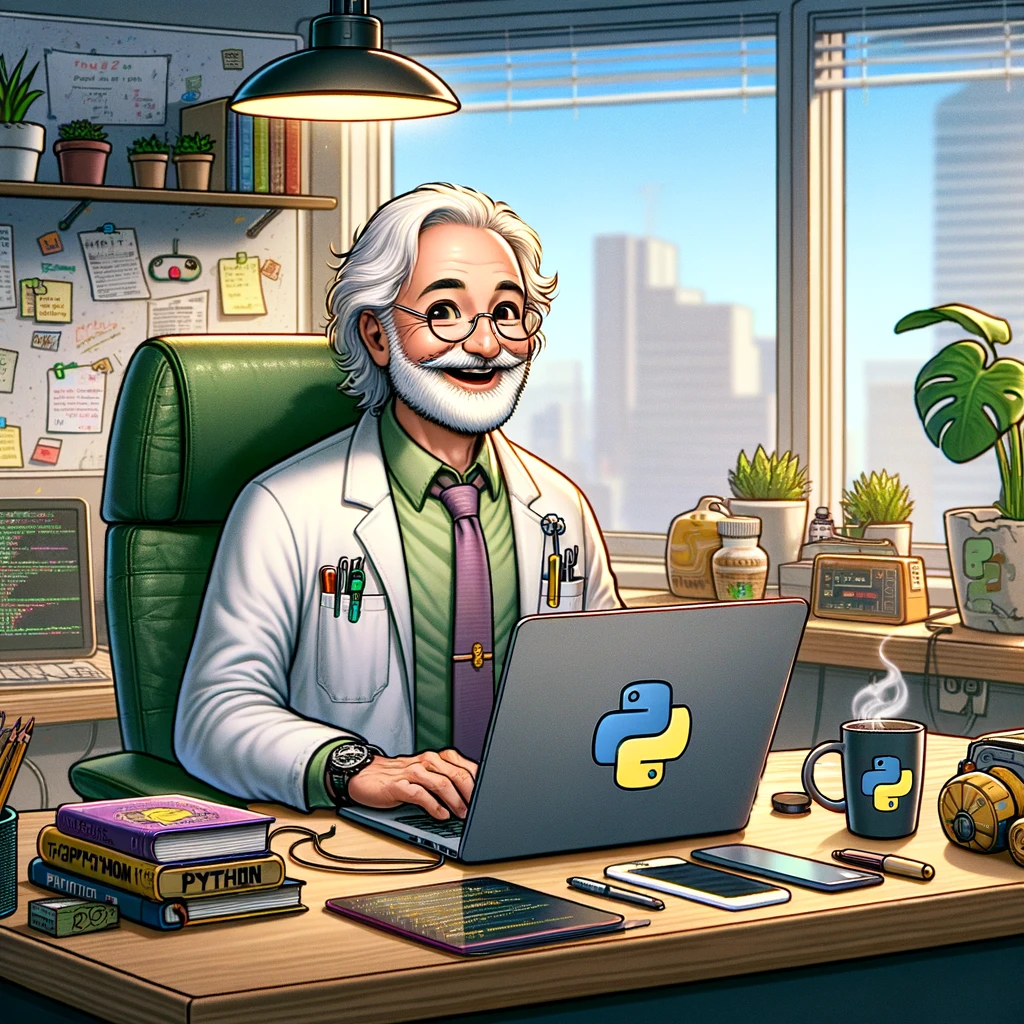
\includegraphics[width=0.35\textwidth]{bob_enlightened.png}
    \end{center}

    In this moment, Bob became enlightened and never wrote Fortran code again.

    Borrowed from a blog post by \href{https://cerfacs.fr/coop/fortran-vs-python}{Centre Europeen de Recherche et Formation Avancee en Calcul Scientifique}

\end{frame}


\section{Layers of scientific Python}
\begin{frame}
    \frametitle{The layers of scientific Python}

    I view there being 5 main layers of scientific Python

    \begin{enumerate}
        \item Core Python
        \item Numeric infrastructure
        \item Scientific infrastructure
        \item General scientific tools
        \item Domain specific tools
    \end{enumerate}

\end{frame}

\begin{frame}
    \frametitle{Scientific Python landscape}

    \begin{center}
        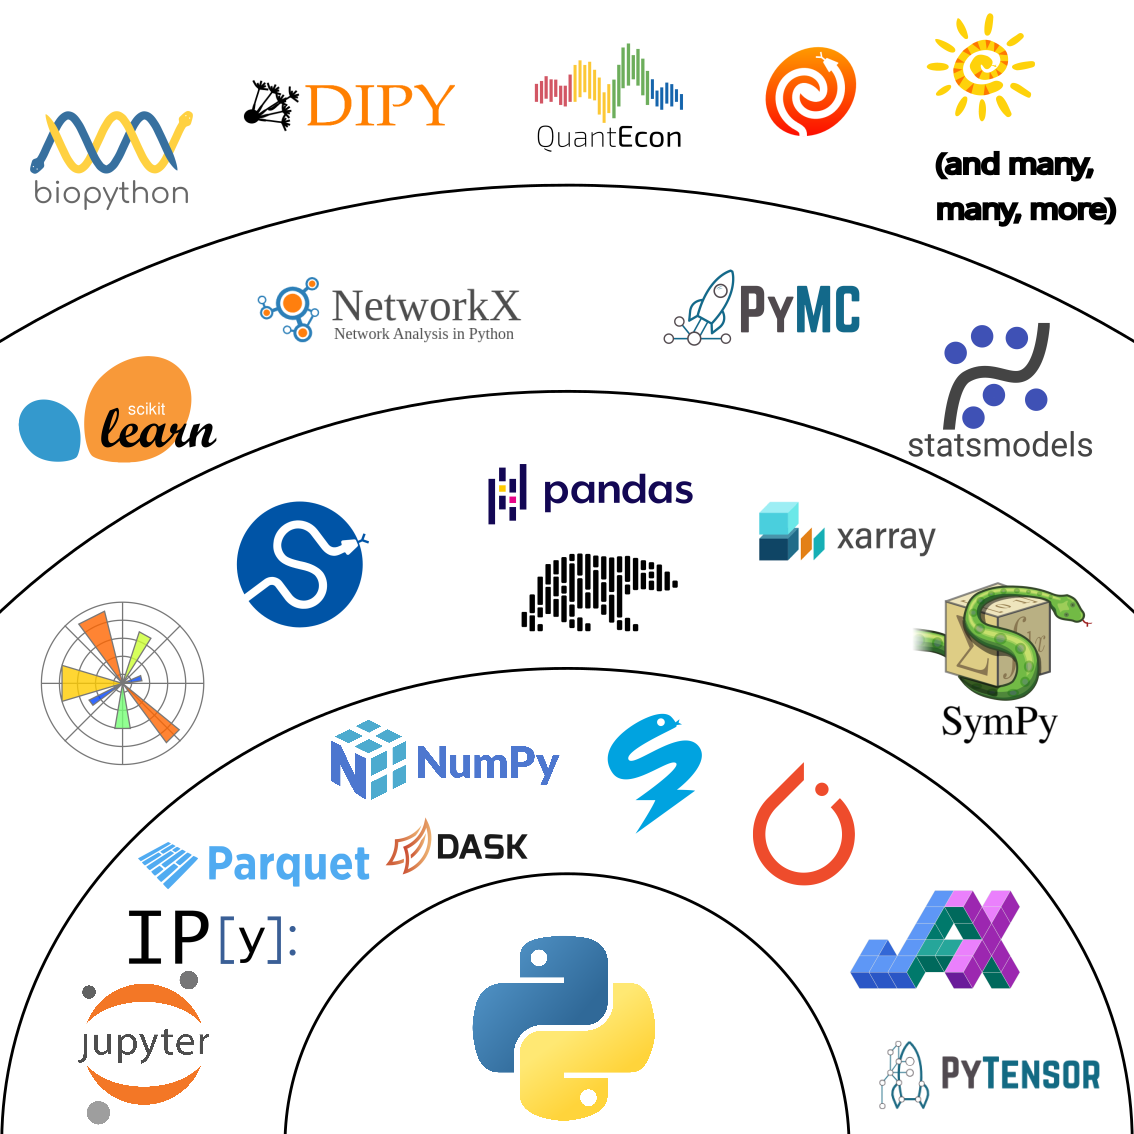
\includegraphics[width=0.75\textwidth]{python_landscape.png}
    \end{center}

\end{frame}

\begin{frame}[fragile]
    \frametitle{Scientific Python: Core Python}

    The entire scientific stack in Python begins with ``core Python'' which includes the standard
    library of Python packages.

    \begin{minted}{python}
import math

x = 2 * math.pi
y = 1.0 / x * math.sin(x)
    \end{minted}

\end{frame}

\begin{frame}[fragile]
    \frametitle{Scientific Python: Numeric infrastructure}

    The numeric infrastructure stack expands what is possible within Python by adding additional
    types and packages that you can directly build on. This will include things like NumPy's
    array type

    \begin{minted}{python}
import math

import numpy as np

x = np.linspace(0.01, 2 * math.pi, 50)
y = 1.0 / x * np.sin(x)

x@y
    \end{minted}

\end{frame}

\begin{frame}[fragile]
    \frametitle{Scientific Python: Scientific infrastructure}

    The scientific infrastructure differs from numeric infrastructure because, rather than build
    general numeric tools, it focuses on tools to perform specific actions, such as interpolation
    or optimization.

    This infrastructure often provides the type of ``algorithm legos'' that makes it easy to
    experiment with different algorithms as you solve your problem of interest.

\end{frame}

\begin{frame}[fragile]
    \frametitle{Scientific Python: Scientific infrastructure}
    \begin{minted}{python}
import math

import numpy as np
import scipy.interpolate as interp

x = np.linspace(0.01, 2 * math.pi, 50)
y = 1.0 / x * np.sin(x)

pwci = interp.CubicSpline(x, y)
pwci(math.pi)

    \end{minted}

\end{frame}

\begin{frame}[fragile]
    \frametitle{Scientific Python: General scientific tools}

    General scientific tools are about simplifying the code to do a specific but widely used task.
    For example, a linear regression really should only take a single line of code.

    \begin{itemize}
        \item If you used numeric infrastructure, it might take a couple hundred lines of code
        \item If you used the scientific infrastructure, it might take 10-20 lines of code
    \end{itemize}

\end{frame}

\begin{frame}[fragile]
    \frametitle{Scientific Python: General scientific tools}

    \begin{minted}{python}
import numpy as np
from sklearn.linear_model import LinearRegression

x = np.linspace(0, 100, 50)
y = 2*x + 0.1*np.random.randn(50)

reg = LinearRegression().fit(x, y)

    \end{minted}

\end{frame}

\begin{frame}
    \frametitle{Scientific Python: Domain specific tools}

    The final layer of the scientific Python stack is the tools used for domain expecific
    analysis.

    For example, the code inside of the QuantEcon Python package is all domain specific code and is
    meant to facilitate the type of analysis/modeling that is done by economists.

\end{frame}

\end{document}

